\documentclass[20pt, a1paper, portrait, margin=10mm, innermargin=15mm, blockverticalspace=15mm]{tikzposter}
\usepackage[utf8]{inputenc}
\usepackage{graphicx}
\usepackage{amsmath}
\usepackage{enumitem}
\usepackage{xcolor}

\title{MacraScript: A Language for Macramé Pattern}
\author{Juan Manuel Serrano Rodriguez - 20211020091 \\ Javier Alejandro Sánchez Salamanca - 20201020167}
\institute{Department of Systems Engineering \\ Universidad Francisco José de Caldas}

\usetheme{Basic}
\usecolorstyle{Spain}

\begin{document}
\maketitle

% Usaremos una estructura de tres columnas para un mejor equilibrio
\begin{columns}

    % --- COLUMNA 1: INTRODUCCIÓN Y OBJETIVO ---
    \column{0.32}
    
    \block{Introduction}{
        Macramé is a textile art form based on knotting, but its design process has traditionally lacked specialized digital tools, relying on manual, error-prone methods. Existing graphic design software is not optimized for the constraints of knot-based textiles. MacraScript is a Domain-Specific Language (DSL) created to bridge this gap. It provides a simple, declarative syntax for artisans, designers, and hobbyists to define macramé patterns programmatically, verify their structure, and generate clear visual guides, thus modernizing a traditional craft.
    }

    \block{Goal}{
        The main goal of this work is to design and implement a DSL, MacraScript, capable of simplifying the creation of complex macramé patterns. The research question is: \textit{How can a DSL abstract the complexities of macramé to provide a user-friendly tool for pattern design and visualization?} The expected final product is a compiler that translates MacraScript code into dual graphical outputs: a final pattern preview and a step-by-step knotting diagram.
    }

    % --- COLUMNA 2: SOLUCIÓN, CONCLUSIONES Y BIBLIOGRAFÍA ---
    \column{0.36} % Un poco más ancha para el texto técnico

    \block{Proposed Solution: MacraScript Language and Compiler}{
        We developed an external, declarative DSL with a simple grammar. The language is built around a \texttt{PATTERN} block, which can be \texttt{ALPHA} (for grid-based images) or \texttt{NORMAL} (for geometric knot patterns). The key innovation is the abstraction of knot-pairing logic in Normal patterns; the user only specifies the knot direction (\texttt{LEFT}/\texttt{RIGHT}), and the compiler handles the complex staggered thread pairing.

        The compiler, written in Python, follows a traditional pipeline:
        \begin{itemize}[leftmargin=*]
            \item \textbf{Lexical Analysis:} Converts code into tokens using regular expressions.
            \item \textbf{Syntactic Analysis:} A recursive descent parser validates the token stream against the grammar.
            \item \textbf{Semantic Analysis:} Validates logical rules and translates the abstract pattern definition into concrete knot instructions.
        \end{itemize}
    }
    
    \block{Conclusions}{
        MacraScript successfully demonstrates that a DSL can effectively abstract the complexities of a traditional craft. By providing a simple declarative language, a robust compiler, and dual visualizations, we have created a powerful tool that lowers the barrier to entry for creating complex designs and reduces manual error. The project successfully answers the research question by providing a functional bridge between computational thinking and macramé art.
    }
    
    \block{Bibliography}{
        \begin{enumerate}[label=\arabic*., itemsep=2pt]
            \item Fowler, M. (2010). \textit{Domain-Specific Languages}. Addison-Wesley Professional.
            \item Mernik, M., Heering, J., \& Sloane, A. M. (2005). When and how to develop domain-specific languages. \textit{ACM Computing Surveys (CSUR)}, 37(4), 316-344.
            \item Karner, C. (2005). \textit{Macramé: The craft of knotting}. Schiffer Publishing.
        \end{enumerate}
    }

    % --- COLUMNA 3: SALIDAS VISUALES Y RESULTADOS ---
    \column{0.32}

    \block{Visual Outputs}{
        The compiler generates two distinct visualizations in a Tkinter-based GUI, serving both the design and execution phases of a project.
        \begin{center}
            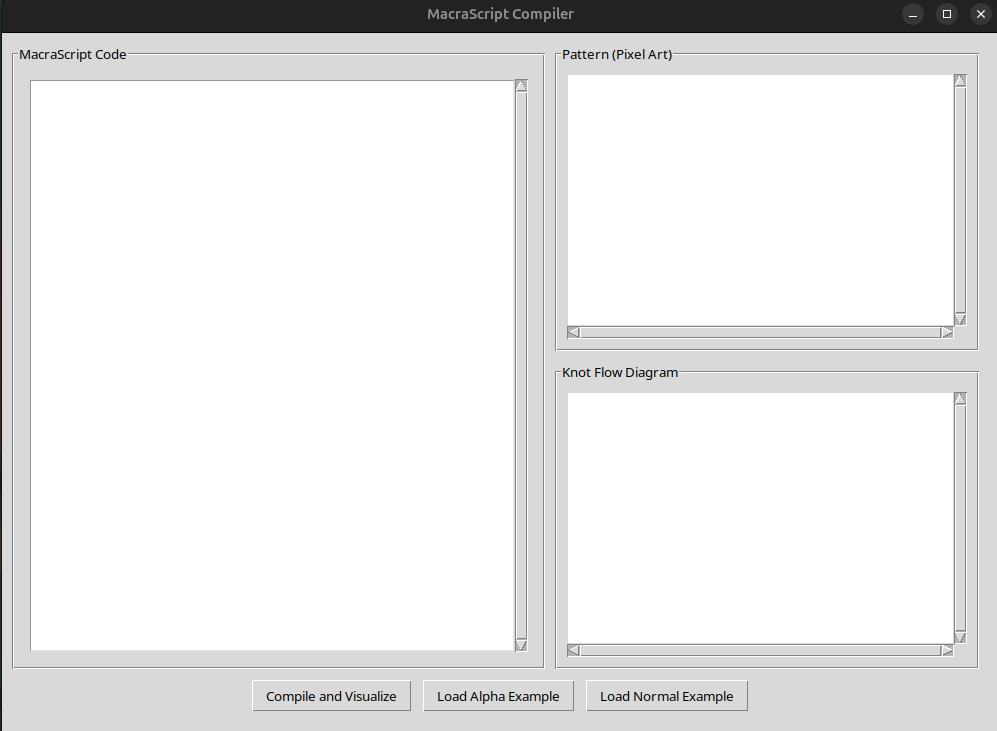
\includegraphics[width=\linewidth]{img/ui_mockup.png} % Ajustado a linewidth
            \note{The MacraScript IDE with its main components.}
        \end{center}
    }

    \block{Experiments and Results}{
        The language was tested with two main types of patterns to validate the compiler and visualization engine. The results confirm that the compiler correctly generates both a final preview and a knot-flow diagram for each pattern type.
        
        % Imágenes más grandes, ocupando más espacio vertical y horizontal
        \begin{center}
            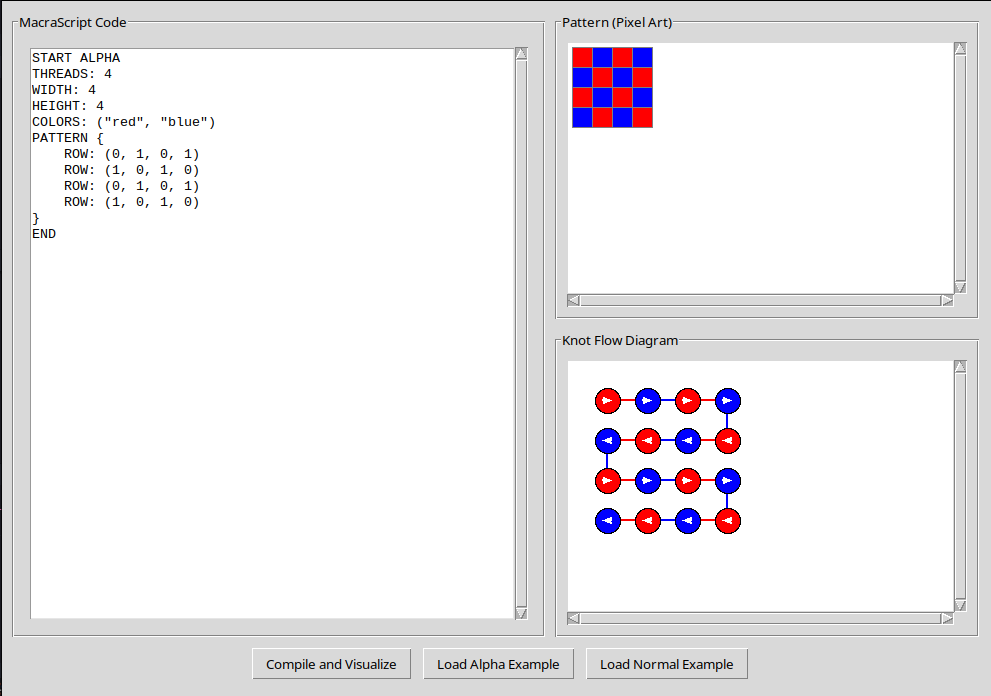
\includegraphics[width=0.7\linewidth]{img/final_alpha_pattern.png}\\[1em]
            \small{\textit{Alpha Pattern Output}}\\[2em]
            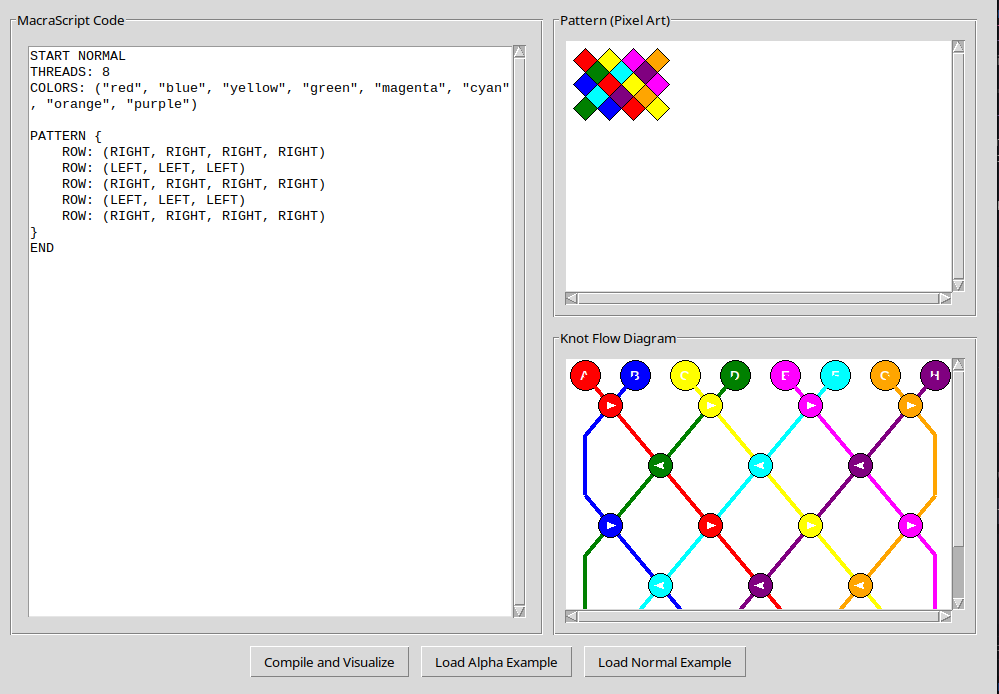
\includegraphics[width=0.7\linewidth]{img/final_normal_pattern.png}\\[1em]
            \small{\textit{Normal Pattern Output}}
        \end{center}
    }

\end{columns}

\end{document}